%------------------------------------------------
\section{Tổng quan}

%------------------------------------------------
\begin{frame}
\label{Maths}
	\frametitle{TỔNG QUAN TẤM PIN NĂNG LƯỢNG MẶT TRỜI}
	\begin{center}
		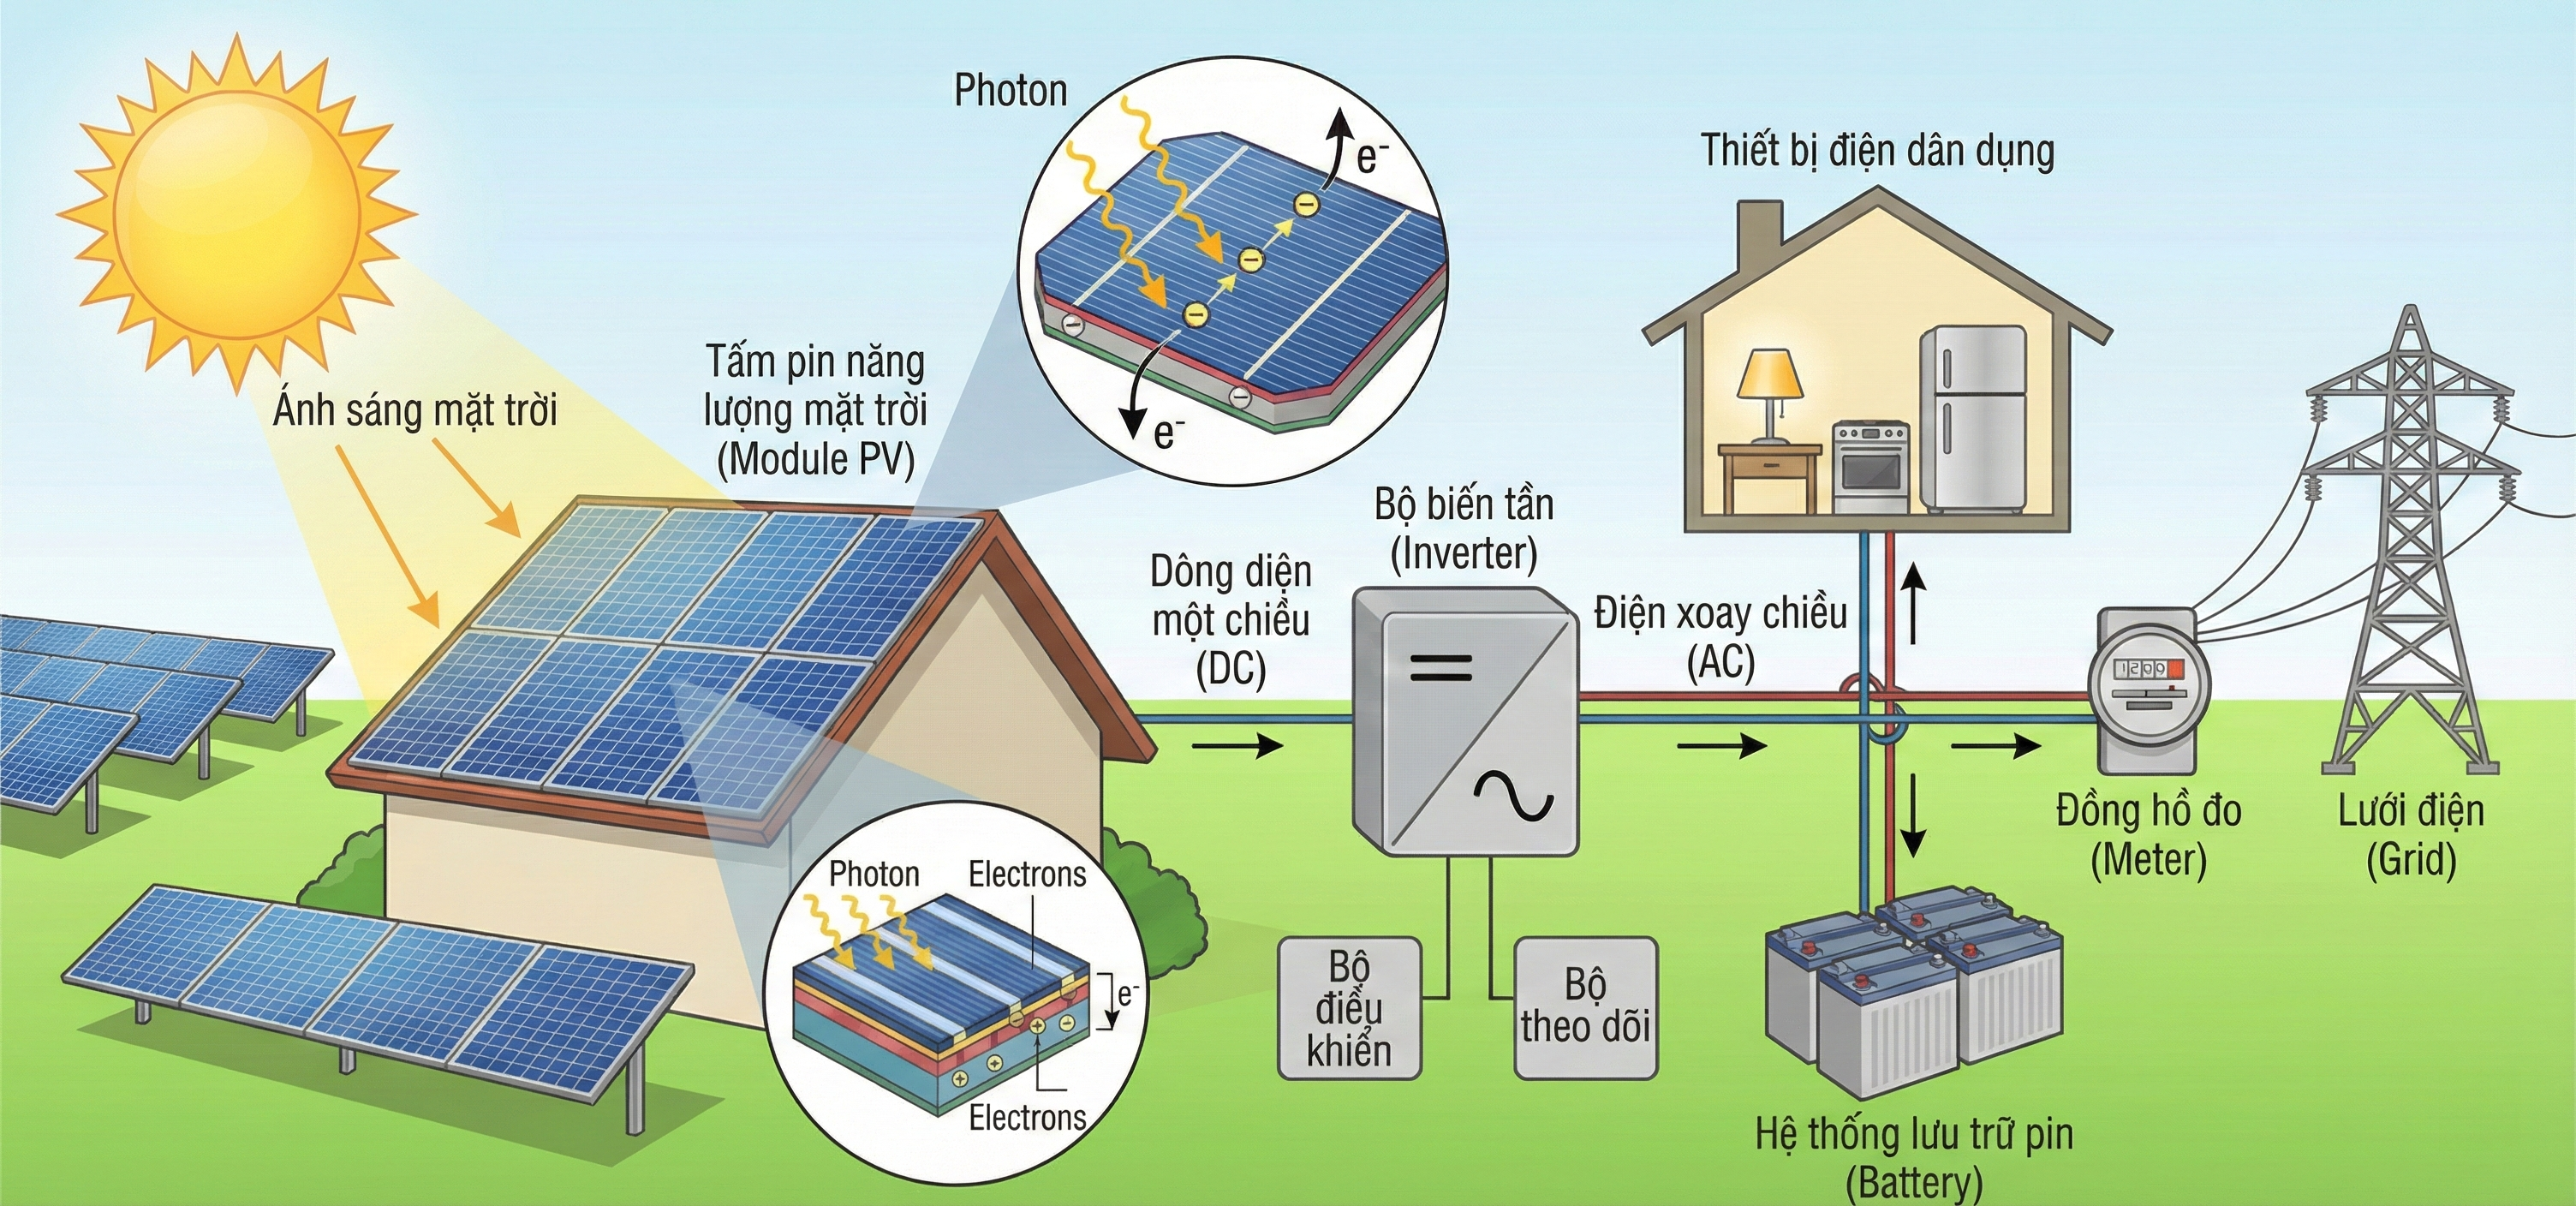
\includegraphics[width=0.8\textwidth]{images/TongQuan/pinmattroi.png}
	\end{center}
\end{frame}

%------------------------------------------------
\begin{frame}
	\frametitle{TÌNH HÌNH HỆ THỐNG PIN MẶT TRỜI TRÊN THẾ GIỚI}
	
	\vspace{0.3cm}
	
	\begin{columns}[t]
		% Cột 1: BÙNG NỔ
		\begin{column}{0.3\textwidth}
			\centering
			\includegraphics[width=0.5\textwidth]{images/TongQuan/icons/bungno.png}
			
			\vspace{0.3cm}
			
			{\Large\textbf{BÙNG NỔ}}
			
			\vspace{0.4cm}
			
			\small
			Diện mặt trời chiếm \\
			\textcolor{orange}{\textbf{73\%}} tổng công suất \\
			năng lượng tái tạo \\
			tăng thêm toàn cầu \\
			năm 2023.
		\end{column}

		\vrule width 1pt
		
		% Cột 2: CHI PHÍ
		\begin{column}{0.3\textwidth}
			\centering
			\includegraphics[width=0.5\textwidth]{images/TongQuan/icons/chiphi.png}
			
			\vspace{0.3cm}
			
			{\Large\textbf{CHI PHÍ}}
			
			\vspace{0.4cm}
			
			\small
			Chi phí lắp đặt đã giảm sâu \\
			\textcolor{orange}{\textbf{85\%}} sau một thập kỷ, trở \\
			thành nguồn năng lượng \\
			dễ tiếp cận nhất.
		\end{column}

		\vrule width 1pt
		
		% Cột 3: TIỀM NĂNG
		\begin{column}{0.3\textwidth}
			\centering
			\includegraphics[width=0.5\textwidth]{images/TongQuan/icons/tiemnang.png}
			
			\vspace{0.3cm}
			
			{\Large\textbf{TIỀM NĂNG}}
			
			\vspace{0.4cm}
			
			\small
			Việt Nam nằm trong \\
			``vùng đỏ'' bức xạ nhiệt, \\
			mang hữu tiềm năng tự \\
			nhiên lý tưởng để phát \\
			triển điện mặt trời.
		\end{column}
	\end{columns}
	
\end{frame}

\begin{frame}
\label{Bungno}
	\frametitle{TÌNH HÌNH HỆ THỐNG PIN MẶT TRỜI TRÊN THẾ GIỚI}
	\begin{center}
		\includegraphics[width=0.7\textwidth]{images/TongQuan/bieudobungno.png}
	\end{center}
\end{frame}

\begin{frame}
\label{Chiphi}
	\frametitle{TÌNH HÌNH HỆ THỐNG PIN MẶT TRỜI TRÊN THẾ GIỚI}
	\begin{center}
		\includegraphics[width=0.6\textwidth]{images/TongQuan/bieudochiphi.png}
	\end{center}
\end{frame}

\begin{frame}
\label{Nhiet}
	\frametitle{TÌNH HÌNH HỆ THỐNG PIN MẶT TRỜI TRÊN THẾ GIỚI}
	\begin{center}
		\includegraphics[width=0.8\textwidth]{images/TongQuan/bieudonhiet.png}
	\end{center}
\end{frame}

\begin{frame}
    \frametitle{TÌNH HÌNH HỆ THỐNG PIN MẶT TRỜI TRÊN VIỆT NAM}
    
    % [FIX 1] Giảm khoảng cách dưới tiêu đề (0.2 -> 0.1)
    \vspace{0.1cm} 
    
    \begin{columns}[T] 
        
        % --- CỘT TRÁI: BẢN ĐỒ ---
        \begin{column}{0.32\textwidth}
            \centering
            \vspace{0pt} 
            \includegraphics[width=0.95\textwidth]{images/TongQuan/bandonhietVietNam.png}
        \end{column}
        
        % --- CỘT PHẢI: NỘI DUNG ---
        \begin{column}{0.65\textwidth}
            \vspace{0pt} 
            
            % === PHẦN 1: PHÁP LÝ ===
            % [FIX 2] Giảm kích thước khung chứa icon (1.2cm -> 0.9cm)
            \begin{minipage}[c]{0.9cm}
                % [FIX 3] Giảm size icon (1.0cm -> 0.75cm) cho gọn
                \includegraphics[width=0.75cm]{images/TongQuan/icons/phaply.png}
            \end{minipage}%
            \hspace{0.1cm}%
            \begin{minipage}[c]{8.8cm} 
                {\Large\textbf{\textcolor{blue!70!black}{PHÁP LÝ}}}
            \end{minipage}
            
            % [FIX 4] Giảm khoảng cách dưới tiêu đề mục (0.1 -> 0.05)
            \vspace{0.05cm}
            
            \footnotesize
            \begin{itemize}
                % [FIX 5] Giảm khoảng cách giữa các item (0.1 -> 0.02)
                \setlength\itemsep{0.02cm} 
                \item Chuyển từ giai đoạn chính sách giá ưu đãi (kích cầu đầu tư ồ ạt) sang giai đoạn phát triển bền vững và có kiểm soát.
                \item Tập trung kiểm soát an toàn lưới điện và đặc biệt ưu tiên khuyến khích mô hình điện mặt trời \textbf{tự sản tự tiêu} (thay vì bán lên lưới).
            \end{itemize}
            
            % [FIX 6] Giảm khoảng cách lớn giữa 2 phần (0.4 -> 0.25)
            \vspace{0.25cm} 
            
            % === PHẦN 2: TIỀM NĂNG ===
            \begin{minipage}[c]{0.9cm}
                \includegraphics[width=0.75cm]{images/TongQuan/icons/tiemnangVietNam.png}
            \end{minipage}%
            \hspace{0.1cm}%
            \begin{minipage}[c]{8.8cm}
                {\Large\textbf{\textcolor{orange}{TIỀM NĂNG}}}
            \end{minipage}
            
            \vspace{0.05cm}
            
            \footnotesize
            \begin{itemize}
                \setlength\itemsep{0.02cm}
                \item \textbf{Việt Nam} nằm trong nhóm quốc gia có bức xạ mặt trời \textbf{tốt nhất Đông Nam Á}, đặc biệt tại miền Trung và Nam Bộ (bức xạ $>$4.6 kWh/kWp/ngày; $>$2500 giờ nắng/năm).
                \item \textbf{Miền Nam} phù hợp phát triển cả trang trại lớn và điện áp mái; \textbf{Miền Bắc} tuy bức xạ thấp hơn nhưng vẫn hiệu quả cho mô hình áp mái kết hợp lưu trữ.
            \end{itemize}
            
        \end{column}
    \end{columns}
\end{frame}

% Định nghĩa màu nền xanh
\definecolor{CardBlue}{HTML}{B1CDFC}

\begin{frame}[shrink=5]
    \frametitle{TÌNH HÌNH HỆ THỐNG PIN MẶT TRỜI TẠI VIỆT NAM}
    
    % Giảm khoảng cách dưới tiêu đề để tiết kiệm không gian
    \vspace{-0.3cm}
    
    \begin{columns}[t, onlytextwidth] % onlytextwidth giúp căn lề chuẩn hơn
        
        % Thiết lập style chung cho các card để code gọn gàng
        \tcbset{
            mycardstyle/.style={
                colback=CardBlue,       % Yêu cầu 3: Full nền xanh
                colframe=CardBlue!80!black, % Viền đậm hơn chút cho đẹp (hoặc để CardBlue nếu muốn ẩn)
                arc=8pt,                % Bo góc box
                boxrule=0pt,            % Bỏ viền dày
                left=2pt, right=2pt, top=2pt, bottom=2pt, % Tối ưu lề (Yêu cầu 1: giảm overfull)
                equal height group=A,   % Yêu cầu 4: Ép 3 cột cao bằng nhau
                fontupper=\tiny,        % Set font chữ nhỏ toàn bộ
                halign=center,          % Căn giữa nội dung
                valign=top              % Căn nội dung từ trên xuống
            }
        }

        % --- Card 1 ---
        \begin{column}{0.32\textwidth}
            \begin{tcolorbox}[mycardstyle]
                % Icon + Tiêu đề
                \includegraphics[height=0.8cm]{images/TongQuan/icons/dienmattroiquymolon.png}
                \par\vspace{0.1cm}
                {\scriptsize\textbf{ĐIỆN MẶT TRỜI\\QUY MÔ LỚN}}
                
                \vspace{0.1cm}
                % Nội dung (căn trái)
                \begin{flushleft}
                    \textbullet\ Nguồn cung cấp sản lượng điện lớn đóng góp vào lưới điện quốc gia.\\[0.1cm]
                    \textbullet\ Các dự án kỷ lục: nhà máy Dầu Tiếng, tổ hợp Trung Nam.
                \end{flushleft}
                
                \vfill % Đẩy ảnh xuống đáy (Yêu cầu 4)
                
                % Yêu cầu 2: Ảnh bo góc bằng TikZ Clip
                \begin{tikzpicture}
                    \clip [rounded corners=6pt] (0,0) rectangle (\linewidth, 1.8cm); 
                    \node[anchor=south west, inner sep=0] at (0,0) {\includegraphics[width=\linewidth, height=1.8cm]{images/TongQuan/trungnam.jpg}};
                \end{tikzpicture}
            \end{tcolorbox}
        \end{column}

        % --- Card 2 ---
        \begin{column}{0.32\textwidth}
            \begin{tcolorbox}[mycardstyle]
                \includegraphics[height=0.8cm]{images/TongQuan/icons/dienmattroiapmai.png}
                \par\vspace{0.1cm}
                {\scriptsize\textbf{ĐIỆN MẶT TRỜI\\ÁP MÁI}}
                
                \vspace{0.1cm}
                \begin{flushleft}
                    \textbullet\ Tận dụng mái nhà xưởng và hộ gia đình.\\[0.1cm]
                    \textbullet\ Ưu tiên hàng đầu: không tốn đất, giảm tải tại chỗ cho lưới điện.
                \end{flushleft}
                
                \vfill
                
				\vspace{0.3cm}
                \begin{tikzpicture}
                    \clip [rounded corners=6pt] (0,0) rectangle (\linewidth, 1.8cm);
                    \node[anchor=south west, inner sep=0] at (0,0) {\includegraphics[width=\linewidth, height=1.8cm]{images/TongQuan/apmai.png}};
                \end{tikzpicture}
            \end{tcolorbox}
        \end{column}

        % --- Card 3 ---
        \begin{column}{0.32\textwidth}
            \begin{tcolorbox}[mycardstyle]
                \includegraphics[height=0.8cm]{images/TongQuan/icons/dienmattroidoclap.png}
                \par\vspace{0.1cm}
                {\scriptsize\textbf{ĐIỆN MẶT TRỜI\\ĐỘC LẬP}}
                
                \vspace{0.1cm}
                \begin{flushleft}
                    \textbullet\ Khu vực chưa có điện lưới hoặc công trình độc lập.\\[0.1cm]
                    \textbullet\ Cần tính toán kỹ pin lưu trữ để đảm bảo ổn định.
                \end{flushleft}
                
                \vfill
                
                \begin{tikzpicture}
                    \clip [rounded corners=6pt] (0,0) rectangle (\linewidth, 1.8cm);
                    \node[anchor=south west, inner sep=0] at (0,0) {\includegraphics[width=\linewidth, height=1.8cm]{images/TongQuan/doclap.png}};
                \end{tikzpicture}
            \end{tcolorbox}
        \end{column}
        
    \end{columns}
    
    \vspace{0.1cm}
    \centering
    \fcolorbox{black!10}{white}{
    \parbox{0.95\textwidth}{
        \tiny \textbf{Tổng kết:} Sự cộng hưởng giữa tiềm năng bức xạ dồi dào và hành lang pháp lý khuyến khích tự sản tự tiêu tạo nền tảng vững chắc để Việt Nam phát triển năng lượng mặt trời hiệu quả và bền vững.
    }}
\end{frame}

%------------------------------------------------
\section{Testing}

%------------------------------------------------
\begin{frame}
	\frametitle{Blocks}
    	\begin{block}{Block Title}
    		Block 1
    	\end{block}
    	
    	\begin{exampleblock}{Example Block Title}
    		Block 2
    	\end{exampleblock}
    	
    	\begin{alertblock}{Alert Block Title}
    		Block 3
    	\end{alertblock}
    	
    	\begin{block}{}
    		Block without a title
    	\end{block}
\end{frame}
